\documentclass[11pt,a4paper]{article}
\usepackage[margin=2cm]{geometry}
\usepackage{mathptmx}
\usepackage[T1]{fontenc}
\usepackage{tabularx,booktabs,array,enumitem,xcolor,tikz,fancyhdr,hyperref}
\usetikzlibrary{positioning}
\hypersetup{hidelinks}
\setlength{\parindent}{0pt}\setlength{\parskip}{4pt}
\renewcommand{\arraystretch}{1.25}
\pagestyle{fancy}\fancyhf{}
\fancyhead[L]{\small KSCST -- SPP 50th Series (2026--27) Project Proposal}
\fancyfoot[C]{\small Page \thepage}
\newcommand{\todo}[1]{\textcolor{red}{[#1]}}
\newcommand{\psec}[1]{\vspace{4pt}\noindent{\large\bfseries #1}\par\vspace{1pt}\hrule\vspace{4pt}}

\begin{document}

\begin{center}
{\Large\bfseries KARNATAKA STATE COUNCIL FOR SCIENCE AND TECHNOLOGY}\\[2pt]
{\bfseries Student Project Programme (SPP) -- 50th Series, 2026--2027}\\[2pt]
{\large\bfseries PROJECT PROPOSAL}
\end{center}

\psec{PART A: GENERAL INFORMATION}

\textbf{Project title:} MandiSense AI: Calibrated Price Forecasting and Sell-or-Hold Advice for Farmers of the Bengaluru--Kolar Belt

\textbf{Keywords:} agricultural price forecasting; APMC mandi; prediction intervals; decision support for farmers; sale planning; Kannada interface; evidence-gated advice

\textbf{Broad theme / sub-theme:} Agriculture and allied sectors -- digital agriculture and AI-based decision support \todo{confirm exact theme wording against the KSCST themes list}

\subsection*{Institution details}
\begin{tabularx}{\textwidth}{@{}lX@{}}
Institution & B.M.S. College of Engineering (Autonomous, affiliated to VTU)\\
Course / Department & B.E. -- Department of Computer Science and Engineering (Data Science)\\
Address & Bull Temple Road, Basavangudi, Bengaluru -- 560019, Karnataka\\
District & Bengaluru Urban\\
\end{tabularx}

\subsection*{Project guide}
\begin{tabularx}{\textwidth}{@{}lX@{}}
Name and designation & Dr. Kalyan N, Assistant Professor, Dept.\ of CSE (Data Science)\\
Email / Mobile & \todo{email} / \todo{mobile}\\
Co-guide (optional) & \todo{name, designation, email, mobile -- or delete}\\
\end{tabularx}

\subsection*{Student team (maximum four; team leader marked)}
\begin{tabularx}{\textwidth}{@{}c>{\raggedright}p{3.4cm}lllll@{}}
\toprule
Photo & Name (block letters) & USN & Branch / Sem & Category & Mobile & Email\\
\midrule
\todo{photo} & SRIJAN C VACHADMATH \todo{leader?} & 1BM23CD060 & CSE-DS / \todo{sem} & \todo{} & \todo{} & \todo{}\\
\todo{photo} & MANOHARA SALMANI & 1BM23CD035 & CSE-DS / \todo{sem} & \todo{} & \todo{} & \todo{}\\
\todo{photo} & SHREEJITH SHAH & 1BM23CD057 & CSE-DS / \todo{sem} & \todo{} & \todo{} & \todo{}\\
\bottomrule
\end{tabularx}

\textbf{SPP Coordinator:} \todo{name, designation, official SPP email, mobile}

\psec{PART B: PROJECT DESCRIPTION}

\subsection*{1. Background and need}
Farmers around Bengaluru and Kolar who grow tomato, onion, potato and ginger sell through Agricultural Produce Market Committee (APMC) mandis, where prices can swing sharply within days (Kolar tomato rose 12\% in one recent week, and from Rs.\,466 to Rs.\,6,117 per quintal between April and July 2023). A grower deciding whether to harvest today, sell locally, carry the load to a better mandi or store it usually relies on word of mouth or on the previous day's board price. Public portals such as Agmarknet publish historical prices, but they show raw numbers: they give no forward view, do not say how uncertain it is, and are seldom available in Kannada. The consequence is distress selling during gluts and missed gains during shortages.

Existing forecasting tools are mostly built for analysts. They output a single number, hide their reasoning and rarely admit when they cannot tell. A farmer cannot act on a number that cannot be questioned, and a tool that sounds sure when it is not can do real harm.

This project turns recorded mandi prices into a plain answer for a farmer: what the crop is worth today, where it fetches most after transport, and whether waiting is likely to pay, with an honest range for the next week. Its guiding rule is that advice must be earned: a sell-or-hold call is given only for a crop and district where it has been shown, on weeks the system had never seen, to do better than assuming the price will not change. Elsewhere the app shows the price and the likely range and says that it has no dependable call. It is aimed at small and marginal growers in the Bengaluru--Kolar belt, and at farmer-producer organisations that plan collective transport.

\textbf{What is already done, and what this proposal funds.} A working system exists and has been tested on real records. The sponsored work is not to build it but to keep it fed with live data, to make its per-market evidence deeper, and to find out whether farmers actually decide better with it.

\begin{tabularx}{\textwidth}{@{}>{\raggedright\arraybackslash}X>{\raggedright\arraybackslash}X@{}}
\toprule
\textbf{Already built and tested (not requested)} & \textbf{Requested funding supports}\\
\midrule
Real Agmarknet data for 5 districts, 16 mandis and 5 crops, with quality checks; forecasting and range model; the evidence rule that decides where advice is given; the farmer web app in Kannada, Hindi and English with voice input; sale planner, fair-price check, hold-or-rot check, alerts engine and truck-sharing board; 651 automated tests &
Daily live collection of prices under a registered data key and hosting; deeper per-market history before November 2025; monthly re-testing of where advice is earned; SMS or messaging delivery of price alerts; a four-week pilot with at least 20 growers or traders, with their decisions measured against selling the same day; field usability tests in Kannada\\
\bottomrule
\end{tabularx}

\subsection*{2. Review of existing work}
\textbf{Statistical and machine-learning forecasting.} Seasonal-trend decomposition \cite{cleveland1990} and exponential-smoothing and ARIMA families \cite{hyndman2021} remain standard baselines for agricultural prices. Gradient-boosted trees \cite{chen2016} usually do better on tabular lag features. The M4 competition \cite{makridakis2020} showed that combining methods is more reliable than trusting one.

\textbf{Uncertainty.} Quantile regression \cite{koenker1978} yields prediction intervals directly, but most farm-price tools published in India report point errors only.

\textbf{Testing a forecast honestly.} Whether a forecast beats a naive rule is a statistical question. The Diebold--Mariano test \cite{diebold1995}, with its small-sample correction \cite{harvey1997}, compares forecast errors; when many series are tested together, Holm's adjustment \cite{holm1979} stops chance results being reported as findings. These tests are rarely applied in price-advisory tools.

\textbf{Government and commercial platforms.} Agmarknet and the data.gov.in mandi feed provide open price data. Existing mobile advisories largely relay these prices or give generic weather tips.

\textbf{Gaps identified.} (i) Little work delivers calibrated ranges together with a decision rather than a bare forecast. (ii) Published accuracy claims often rest on a single split, with no comparison against a ``tomorrow equals today'' rule and no correction for testing many series. (iii) Kannada-language, voice-friendly access to such analytics is uncommon. (iv) Test data of uncertain origin can inflate apparent accuracy; we found a Karnataka data set that made our own system look about ten times better than it is (Part B, Section 14).

\subsection*{3. Problem statement}
To keep running, and to test with real farmers, a decision-support system that turns mandi price and arrival records into calibrated 3--7 day price ranges and a sell, hold or carry-elsewhere recommendation for farmers of the Bengaluru--Kolar belt, issuing advice only where its record has earned it and declining otherwise.

\subsection*{4. Objectives}
\begin{enumerate}[leftmargin=*,nosep]
\item \textbf{Live data.} Collect Agmarknet prices and arrivals every day for the 16 Karnataka markets and 5 crops under a registered data key, with automatic quality checks. \emph{Target:} at least 95\% of market-days captured over the pilot.
\item \textbf{Deeper per-market history.} Extend verified history before November 2025 for the 16 markets and check it against the district series, so forecasts and the sale planner can be validated per market and not only per district. \emph{Target:} at least two years of verified history for at least 10 markets.
\item \textbf{Evidence-gated advice.} Re-test every month which crop--district series earn a sell-or-hold call, with the same corrected statistical test, and publish every result including the failures. \emph{Target:} raise the number of series with earned advice from 5 of 18, or report why not.
\item \textbf{Alert delivery.} Connect the existing alert engine to an SMS or messaging service for pilot users. \emph{Target:} at least 90\% of triggered alerts delivered.
\item \textbf{Field pilot.} Run a four-week pilot with at least 20 growers or traders around Kolar and Chikkaballapur using the sale planner, and compare each followed plan with selling the same day, using recorded mandi prices rather than self-reports. \emph{Target:} report the mean gain or loss in rupees per load, with its uncertainty.
\item \textbf{Usability in Kannada.} After one use, test whether participants can say what their crop is worth and whether waiting is likely to pay. \emph{Target:} at least 80\% correct.
\end{enumerate}

\subsection*{5. Innovation and novelty}
\begin{itemize}[leftmargin=*,nosep]
\item \textbf{Advice that has to be earned:} a sell-or-hold call is shown only for crop--district series whose gain over ``no change'' survives a corrected statistical test; five of eighteen series pass today, and the app says so plainly for the rest.
\item \textbf{Uncertainty drawn as a shape:} the next week's price is a corridor that widens with the days, so a farmer sees how far to trust the forecast without reading a number.
\item \textbf{A sale planner with safeguards:} it never recommends a mandi too small to take the load, a price out of line with neighbouring mandis, or a haul too long for a crop that spoils; every figure is in rupees, on one footing.
\item \textbf{Two data layers:} a long district history for the forecast, and each mandi's own minimum, typical and maximum price each day for where-to-sell and fair-price checks.
\item \textbf{A data-integrity audit:} we showed that a synthetic Karnataka data set can make a forecasting system look ten times better than it is, and built the system so no such data can reach a farmer.
\item \textbf{Built for the farmer:} Kannada, Hindi and English with voice input, a crop-first layout, and a record of how often the system has been right shown on the home page.
\end{itemize}

\subsection*{6. Proposed methodology}

\begin{center}
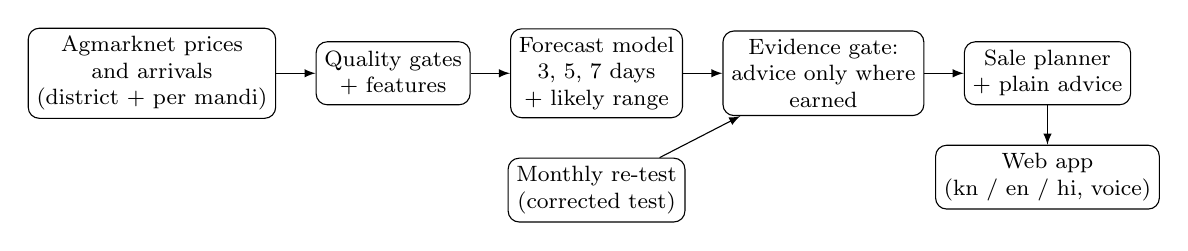
\begin{tikzpicture}[node distance=5mm,
 b/.style={draw,rounded corners,align=center,minimum height=8mm,font=\footnotesize,inner sep=3pt},
 a/.style={-latex}]
\node[b](d){Agmarknet prices\\and arrivals\\(district + per mandi)};
\node[b,right=of d](q){Quality gates\\+ features};
\node[b,right=of q](m){Forecast model\\3, 5, 7 days\\+ likely range};
\node[b,right=of m](r){Evidence gate:\\advice only where\\earned};
\node[b,right=of r](p){Sale planner\\+ plain advice};
\node[b,below=5mm of m](t){Monthly re-test\\(corrected test)};
\node[b,below=5mm of p](u){Web app\\(kn / en / hi, voice)};
\draw[a](d)--(q);\draw[a](q)--(m);\draw[a](m)--(r);\draw[a](r)--(p);
\draw[a](t)--(r);\draw[a](p)--(u);
\end{tikzpicture}\\
{\small Figure 1. Overall architecture.}
\end{center}

\textbf{Step 1 -- Data.} Two real Agmarknet sources are kept in separate tables: the district report (one arrivals-weighted price and arrivals total per district, crop and day, from January 2021) and the per-mandi reports (minimum, typical and maximum price and arrivals, from November 2025). Records pass quality checks (impossible prices, gaps, stale series); a series needs enough history and a recent print to be forecast.

\textbf{Step 2 -- Features and model.} Price lags and rolling statistics, arrival volumes, calendar and seasonal features feed gradient-boosted trees that predict the change in log-price at 3, 5 and 7 days. The 1-day horizon is not offered: it was no better than assuming no change. A second set of quantile models gives the likely range.

\textbf{Step 3 -- Evidence gate.} For each crop--district series, the model's out-of-sample errors are compared with ``the price will not change'' using a Diebold--Mariano test, adjusted for testing all series together. Only series that pass receive a sell-or-hold call; the others show price and range.

\textbf{Step 4 -- Sale planner.} For a load of a given size, the planner compares selling at the farmer's own mandi, carrying it to another mandi (after a stated transport rate), and, where advice has been earned, waiting (after the crop's daily spoilage). It excludes mandis too small for the load or priced out of line with their neighbours, and limits the haul for crops that spoil fast.

\textbf{Step 5 -- Evaluation.} Walk-forward tests: the model is fitted on the past, scored on the weeks after, and moved forward four times; gain over the naive rule with confidence intervals; coverage of the 90\% range; precision of sell and hold calls against base rates; and a forward test of a model frozen in February 2025. In the pilot, each followed plan is compared with the same-day price.

\textbf{Software specification.} Python 3.11, FastAPI, pandas, scikit-learn, XGBoost, statsmodels; Next.js with TypeScript and Tailwind for the interface; Docker for deployment. No special hardware is needed.

\subsection*{7. Expected deliverables}
Working web application and REST API running on live data; the validated forecasting model with a reproducible build and evaluation script; a cleaned, documented Karnataka mandi data set; the farmer interface in Kannada, English and Hindi with voice input; alert delivery by SMS or messaging; pilot report; technical report and poster for the state-level exhibition.

\subsection*{8. Expected outcomes and impact}
\textbf{Technical:} forecasts with ranges whose coverage is measured, and advice only where it has been shown to beat the naive rule. \textbf{Social and economic:} better timing and choice of market for small growers, with the gain measured in rupees from recorded prices. \textbf{Academic:} an open, reproducible benchmark for Indian mandi forecasting, and evidence on how often advice can be earned. \textbf{Users:} farmers, farmer-producer organisations, APMC officials and extension workers.

\subsection*{9. Relevance}
[X] Agriculture \quad [X] Rural development \quad [X] Digital India \quad [X] Karnataka priority sectors \quad [X] SDG 1, 2 and 12 \quad [\ ] others

\subsection*{10. Work plan (5 months)}
\begin{tabularx}{\textwidth}{@{}Xccccc@{}}
\toprule
Activity & M1 & M2 & M3 & M4 & M5\\
\midrule
Registered data key, hosting and daily live collection & $\bullet$ & $\bullet$ & & &\\
Extend per-market history before Nov 2025 and verify it & $\bullet$ & $\bullet$ & $\bullet$ & &\\
Monthly re-test of where advice is earned & & $\bullet$ & $\bullet$ & $\bullet$ & $\bullet$\\
SMS or messaging delivery of alerts & & & $\bullet$ & &\\
Pilot preparation: consent, farmer organisations, training & & & $\bullet$ & $\bullet$ &\\
Four-week pilot and usability tests & & & & $\bullet$ & $\bullet$\\
Analysis, final report, poster and exhibition preparation & & & & & $\bullet$\\
\bottomrule
\end{tabularx}

\subsection*{11. Available facilities}
Institutional computing laboratory and campus network of the department; personal laptops of the team; open-source software only; cloud free tier for hosting during development. \todo{confirm with guide/HoD}

\subsection*{12. Major requirements}
Software: Python stack and Next.js listed in Section 6 (all open source). Cloud hosting and domain for the pilot. Travel for mandi visits and farmer meetings at Kolar and Chikkaballapur yards. Alert delivery service (SMS or messaging) for the pilot. Printing of poster and survey forms. No hardware or consumables are required.

\subsection*{13. Budget estimate}
\begin{tabularx}{\textwidth}{@{}lXr@{}}
\toprule
Head & Description & Amount (Rs.)\\
\midrule
Software / cloud services & Hosting and domain for live deployment & 3,000\\
Field survey / data collection & Travel to Kolar and Chikkaballapur yards; farmer meetings; pilot sessions & 3,500\\
Testing / analysis & SMS or messaging service for alerts during the pilot & 1,500\\
Printing & Survey forms, consent forms, poster & 1,000\\
Miscellaneous & Contingency & 1,000\\
Equipment / components, consumables, fabrication & Not required & 0\\
\midrule
\multicolumn{2}{@{}l}{\textbf{Total project budget (within the Rs.\,10,000 ceiling)}} & \textbf{10,000}\\
\bottomrule
\end{tabularx}

\subsection*{14. Preliminary results already achieved}
The system was built and tested before this proposal, on real Agmarknet records only. The data are the district report for five districts around Bengaluru (tomato, onion, potato, ginger, garlic; January 2021 to September 2026; 22,928 daily prices in 18 series) and per-mandi reports for 16 mandis from November 2025 (5,707 prices). Gain is the reduction in average error against ``the price will not change''; every figure is measured on weeks the model had not seen (four expanding test windows, 44,534 forecasts), with 95\% confidence intervals from block resampling.

\begin{tabularx}{\textwidth}{@{}Xcccc@{}}
\toprule
Horizon & 1 day & 3 days & 5 days & 7 days\\
\midrule
Gain over ``no change'' & +0.2\% & +3.0\% & +3.5\% & +3.1\%\\
95\% interval & $-$1.7 to +1.6 & 1.6 to 4.2 & 2.2 to 4.7 & 1.8 to 4.2\\
Direction of the move read right & 62\% & 62\% & 61\% & 60\%\\
Real price inside the 90\% range & 90.1\% & 89.9\% & 89.8\% & 89.5\%\\
Sell calls beat the base rate by & 1.30$\times$ & 1.31$\times$ & 1.28$\times$ & 1.29$\times$\\
Hold calls beat the base rate by & 1.17$\times$ & 1.19$\times$ & 1.21$\times$ & 1.21$\times$\\
\bottomrule
\end{tabularx}

\textbf{Forward test.} A model fitted once on an older real archive, frozen at 7 February 2025 and never refitted, kept its gain on the 20 months that followed: +4.9\%, +5.0\% and +3.8\% at 3, 5 and 7 days for Kolar tomato, and +4.2\%, +4.6\% and +3.0\% for the other district series, all with intervals above zero.

\textbf{Where advice is earned.} Of the 18 crop--district series, 5 show a gain that survives correction for testing all of them: Kolar potato (+13\%), Chikkaballapur potato, onion and tomato, and Kolar ginger. Ten are undetermined, including Kolar tomato (+3.4\%, not significant after correction), and three are worse than assuming no change (Bengaluru garlic, potato and Bengaluru Rural onion). The app gives sell-or-hold calls only for the five.

\textbf{Honest scope statement.} Prices are hard to predict: a gain of about 3 per cent is small, and the 1-day forecast is not offered. The district prices are averages over each district's mandis, not single markets, so the system is validated per district; per-market validation needs the deeper history asked for here. The Kolar tomato series overlaps an older study of the same market before January 2025. Which series receive advice was decided on the same test windows, so the per-series gains are somewhat flattering. A Karnataka data set of 15 mandis that we first used for interface development was found to be synthetic: it does not match the real Kolar prices (correlation $-0.37$) and misses the July 2023 tomato spike, and one annual sine wave explains 92--93\% of its price variance against 0.5--9\% for real series. It made our system look about ten times more accurate than it is, so it is no longer used anywhere in the farmer app. In a cross-commodity analysis, one of forty candidate links passed the first tests and none survived a permutation check, so no link is claimed. No farmer has yet used the system in the field; that is the pilot.

\textbf{Implemented modules:} real-data pipeline with quality gates; forecasting and range model; evidence gate; sale planner; fair-price check, hold-or-rot check, supply (arrivals) signal, last-year comparison and crop-planning tools; price alerts and truck-sharing board; farmer web application in three languages with voice; an accuracy page that shows the record including failures; containerised deployment; and an automated test suite of 651 passing tests.

\subsection*{15. References}
\begin{thebibliography}{9}\small
\bibitem{chen2016} T. Chen and C. Guestrin, ``XGBoost: A scalable tree boosting system,'' in \emph{Proc. 22nd ACM SIGKDD Int. Conf. Knowledge Discovery and Data Mining}, 2016, pp. 785--794.
\bibitem{cleveland1990} R. B. Cleveland, W. S. Cleveland, J. E. McRae and I. Terpenning, ``STL: A seasonal-trend decomposition procedure based on loess,'' \emph{J. Official Statistics}, vol. 6, no. 1, pp. 3--73, 1990.
\bibitem{koenker1978} R. Koenker and G. Bassett, ``Regression quantiles,'' \emph{Econometrica}, vol. 46, no. 1, pp. 33--50, 1978.
\bibitem{makridakis2020} S. Makridakis, E. Spiliotis and V. Assimakopoulos, ``The M4 competition: 100,000 time series and 61 forecasting methods,'' \emph{Int. J. Forecasting}, vol. 36, no. 1, pp. 54--74, 2020.
\bibitem{hyndman2021} R. J. Hyndman and G. Athanasopoulos, \emph{Forecasting: Principles and Practice}, 3rd ed. Melbourne: OTexts, 2021.
\bibitem{diebold1995} F. X. Diebold and R. S. Mariano, ``Comparing predictive accuracy,'' \emph{J. Business \& Economic Statistics}, vol. 13, no. 3, pp. 253--263, 1995.
\bibitem{harvey1997} D. Harvey, S. Leybourne and P. Newbold, ``Testing the equality of prediction mean squared errors,'' \emph{Int. J. Forecasting}, vol. 13, no. 2, pp. 281--291, 1997.
\bibitem{holm1979} S. Holm, ``A simple sequentially rejective multiple test procedure,'' \emph{Scandinavian J. Statistics}, vol. 6, no. 2, pp. 65--70, 1979.
\bibitem{agmarknet} Government of India, Agmarknet portal, Directorate of Marketing and Inspection, and Open Government Data Platform India (data.gov.in), daily mandi price datasets.
\end{thebibliography}

\vspace{8pt}
\psec{SIGNATURES}
\begin{tabularx}{\textwidth}{@{}Xlll@{}}
\toprule
Student name & USN & Signature & Date\\
\midrule
Srijan C Vachadmath & 1BM23CD060 & & \\
Manohara Salmani & 1BM23CD035 & & \\
Shreejith Shah & 1BM23CD057 & & \\
\bottomrule
\end{tabularx}

\vspace{1.2cm}
\begin{tabularx}{\textwidth}{@{}XXXX@{}}
\rule{3.5cm}{0.4pt} & \rule{3.5cm}{0.4pt} & \rule{3.5cm}{0.4pt} & \rule{3.5cm}{0.4pt}\\
Project Guide\newline Dr. Kalyan N (seal) & SPP Coordinator\newline (seal) & Head of Department\newline Dr. Shambhavi B R (seal) & Principal\newline Dr. Bheemsha Arya (seal)\\
\end{tabularx}

\end{document}
